\documentclass[11pt]{article}
\usepackage[margin=1in]{geometry}
\usepackage{graphicx}
\usepackage{fancyhdr}
\usepackage{titling}
\usepackage{enumitem}
\PassOptionsToPackage{hyphens}{url}\usepackage{hyperref}
\usepackage{xcolor}
\usepackage{amsmath}
\usepackage{amssymb}
\usepackage{booktabs}
\usepackage{tabularx}
\usepackage[most]{tcolorbox}
\usepackage{caption}
\captionsetup{font=footnotesize, labelfont=bf, labelsep=period}

\setlength{\headheight}{40pt}
\setlength{\headsep}{20pt}

\hypersetup{colorlinks=true, urlcolor=blue, linkcolor=black, citecolor=black, pdfborder={0 0 0}}

\pagestyle{fancy}
\fancyhf{}
\lhead{
\includegraphics[height=1.4cm]{logo.png}}
\rhead{\small \textsf{Schmidt Sciences \\ Astrophysics Institute}}
\cfoot{\thepage}

\pretitle{\vspace{1cm}\begin{center}\LARGE\bfseries}
\posttitle{\par\end{center}\vskip 1.5em}
\preauthor{\begin{center}\large\lineskip 0.5em\begin{tabular}[t]{c}}
\postauthor{\end{tabular}\end{center}}
\predate{\begin{center}\large}
\postdate{\end{center}}

\newcommand{\docidprefix}{SM\_00X\_Lazuli}
\newcommand{\observatory}{Lazuli}
\newcommand{\Ha}{H$\alpha$}
\newcommand{\ergcgs}{erg~s$^{-1}$~cm$^{-2}$}

\title{\observatory\ Science Memo: Feasibility of \Ha\ High-Contrast Imaging of Accreting Protoplanets with the WCC, and its Sensitivity to Jitter and Strehl Ratio}
\author{Gudmundur Stefansson \\}
\date{2026 September 19}

\begin{document}
\maketitle
\thispagestyle{fancy}

\begin{center}
\begin{tcolorbox}[colback=gray!10!white, colframe=gray!50!black, boxrule=0.5pt, width=0.9\textwidth]
\centering
\textbf{Content marked for:} \textcolor{red}{\textbf{Internal Only}} / \textcolor{teal}{External Use}
\end{tcolorbox}
\end{center}

\begin{center}
\textbf{Document ID:} \texttt{\docidprefix}
\end{center}

\vspace{1em}
\noindent
\textbf{Document Version History}
\vspace{0.5em}

\begin{tabular}{|p{1.3cm}|p{2.2cm}|p{2.2cm}|p{4.2cm}|p{3.8cm}|}
\hline
\textbf{Version} & \textbf{Date} & \textbf{Authors} & \textbf{Change Description} & \textbf{Approved By / Date} \\
\hline
0.1 & 2026-09-19 & GKS & Initial draft, after an independent adversarial review of the two analysis notebooks & \\
\hline
\end{tabular}

\vspace{1.5em}

% ============================================================================
\section*{Summary of decisions}

The Wide-field Context Camera (WCC) filter wheel carries \Ha\ filters of 2, 6 and 20~nm width. This memo asks whether the WCC can image accreting protoplanets of the PDS~70 class in \Ha, which filter to use, and how the answer depends on pointing jitter (0 to 20~mas), Strehl ratio (1.0 to 0.7) and the stability of the PSF between science and reference observations. It uses the WCC ETC instrument model throughout.

\begin{itemize}[leftmargin=*]
  \item \textbf{The 2~nm filter is the right one, and by more than the photon budget suggests.} The planet is a line and gives the same 0.87~e$^-$~s$^{-1}$ per $10^{-16}$~\ergcgs\ in every filter; the host continuum scales with the filter width. In the photon-noise limit the narrow filter improves the line-flux limit only as the square root of the width (3.1$\times$ over 20~nm), because the saturation-limited frame time shortens with the star's brightness and read noise scales with it. Every PSF-subtraction residual, however, is a fixed fraction of the stellar light, so against systematics the 2~nm filter wins by the full factor 10. The 20~nm filter also loses of order 30\% of the time to readout at its 0.75~s frames.
  \item \textbf{PDS~70~b and c are photon-noise detections within an hour.} With an ideal PSF subtraction the 2~nm filter reaches a signal-to-noise ratio (SNR) of 46 (b, $8.1 \times 10^{-16}$~\ergcgs\ at 160~mas) and 22 (c, $3.1 \times 10^{-16}$ at 210~mas) in 1~h at the baseline PSF (10~mas jitter, $S = 1$), and 31 and 18 at the requirement corner ($S = 0.82$ at \Ha). The 5$\sigma$ line-flux limit in 1~h is $0.8 \times 10^{-16}$~\ergcgs\ at 160~mas and $0.6 \times 10^{-16}$ beyond 300~mas, an order of magnitude below the ground-based MagAO-X contrast at the same separations. The host model is verified against the Hubble Space Telescope (HST) F656N planet-to-star ratio to 6\%.
  \item \textbf{Static jitter and Strehl are a modest effect.} Across the grid the photon limit at 160~mas moves by a factor 0.9 to 2.5 relative to the baseline (1.5 at the requirement corner). The Airy wing already dominates the stellar light at 3 to 5 Airy FWHM; jitter only redistributes it between the rings, and lower Strehl lengthens the frames, which partly offsets the added halo in the read-noise term.
  \item \textbf{Jitter mismatch between science and reference is not a floor.} Its residual is azimuthally symmetric and a radial-profile fit removes it to two orders of magnitude below the planets. Jitter enters this science only through the static blur.
  \item \textbf{Wavefront stability between science and reference sets the floor, and it must be specified in nanometers per spatial-frequency band, not as a Strehl.} A change of the wavefront by a few nm root mean square (RMS) between sequences produces speckles that interfere with the Airy rings and with the static aberration pattern; they are not symmetric and survive a radial fit. The floor is linear in the drift. With a 5$\times$ bias margin, the drift at which the floor equals the flux of PDS~70~b in the 2~nm filter is 3.9~nm RMS for a drift with the same power-law spectrum as the static error at $S = 1$, 1.9~nm at $S = 0.82$, and 1.3~nm if the drift is concentrated at 3 to 5 cycles per aperture, which scatters light directly to the planets' separations. Low-order drift (focus, astigmatism) matters only through the static aberrations it beats against: 150~nm at $S = 1$, 4~nm at $S = 0.82$. Registration between science and reference is a first-order dipole term: 3~mas (0.2~pixel) equals the planet's flux, 0.5~mas is a factor 6 below.
  \item \textbf{Recommendation.} Baseline the 2~nm \Ha\ filter for this science case. Ask engineering for the wavefront repeatability between science and reference sequences (or between the two halves of a roll pair) in nm RMS per spatial-frequency band, with the printed allowed-drift table as the target, and for a bound on near-core scattered light inside 1$^{\prime\prime}$, which the FRED model does not resolve. Ask operations for a reference (or roll) taken in the same thermal state as the science sequence. Jitter at the 10 to 20~mas level and Strehl at the 0.8 level are not what limits this science.
\end{itemize}

% ============================================================================
\section*{Background}

Young giant planets still accreting from their circumstellar disk shine in \Ha. The line is powered by the accretion shock, and the host star is continuum there, so in a narrow filter centered on the line the planet-to-star flux ratio is far more favorable than in any broad band. The benchmark system is PDS~70, a K7 T~Tauri star at 113~pc with two accreting planets inside its transition-disk gap: PDS~70~b at 150 to 180~mas and PDS~70~c at 205 to 240~mas from the star, both detected in \Ha\ from the ground with the Multi Unit Spectroscopic Explorer (MUSE) on the Very Large Telescope and with MagAO-X, and from space with HST (Haffert et al.\ 2019; Hashimoto et al.\ 2020; Zhou et al.\ 2021; Close et al.\ 2025). Their line fluxes are a few $10^{-16}$ \ergcgs\ and vary by factors of a few between epochs (Table~\ref{tab:pds70}). A camera in space with a stable point spread function (PSF) and no atmospheric speckles is a natural instrument for this science, and the WCC filter wheel carries three \Ha\ filters of 2, 6 and 20~nm width whose throughput curves are in the WCC exposure time calculator (ETC).

This memo asks two questions. First, can the WCC, with a 3.065~m aperture, 16.87~mas pixels and a 45~mas diffraction-limited full width at half maximum (FWHM) at 656~nm, detect the PDS~70 planets and the class they represent, and which \Ha\ filter serves the case best? Second, since the answer depends on how well the stellar PSF can be subtracted, how sensitive is it to the delivered pointing jitter (0 to 20~mas, 1$\sigma$ per axis) and Strehl ratio (1.0 to 0.7), and to their stability between science and reference observations? The second question connects to the same requirements discussed in the companion memo on in-focus science versus jitter and Strehl.

All calculations use the \texttt{wcc\_etc} instrument model through the \texttt{wcc\_sim} image simulator and are reproducible from two notebooks in \path{notebooks_scrap/} of the \texttt{wcc-sim} repository (\path{halpha_hci_feasibility.ipynb} and \path{halpha_hci_jitter_strehl.ipynb}, with shared helpers in \path{hci_psf.py}). Both notebooks were reviewed by an independent adversarial pass before this memo was written; the review changed the metric for the subtraction floor and the way filters are compared (see Modeling Approach).

% ============================================================================
\section*{Modeling Approach}

\paragraph{Host and planet.} The host is the ETC's K7V Pickles template normalized to the Gaia $G$ magnitude of PDS~70 ($G = 11.6$; Simbad). The planet is a pure emission line, the ETC's absolute-flux \texttt{emission} source, a Gaussian of 2~\AA\ FWHM at 6563~\AA\ with a prescribed integrated flux, so its detected rate is proportional to the line flux and the same in every filter that contains the line. We verified the host model against HST: the planet-to-star flux ratio implied by the ETC for the Zhou et al.\ (2021) line flux of PDS~70~b, rescaled to the 17.7~\AA\ width of the WFC3 F656N filter, agrees with the ratio measured by HST in that filter (planet $1.62 \times 10^{-15}$, star $1.18 \times 10^{-12}$ \ergcgs) to within a few percent, which also shows that the host's own \Ha\ emission is a small correction for this weak-line T~Tauri star.

\paragraph{Filters.} The three \Ha\ filters are taken from the ETC end-of-life throughput curves for the IMX455 channel (\texttt{zwo:halpha2}, \texttt{zwo:halpha6}, \texttt{zwo:halpha20}). Their equivalent widths are 2.0, 6.0 and 19.4~nm and their peak throughputs are within 3\% of each other (Figure~\ref{fig:filters}), so the planet loses nothing in the core by going narrow while the stellar continuum drops in proportion to the width.

\paragraph{PSF model.} The stellar PSF is the ETC's monochromatic Airy pattern at the source-weighted effective wavelength (656.3~nm), rendered on an 11$\times$ oversampled grid and convolved with a circular Gaussian of width $\sigma_{\rm jit}$ (the ETC's jitter model). To represent a Strehl ratio $S < 1$ we use the core-plus-halo model of the companion memo,
\begin{equation}
  \mathrm{PSF} = S\,\mathrm{Airy}_{\rm jit} + (1 - S)\,G(\sigma_{\rm halo}),\qquad
  \sigma_{\rm halo}^2 = \left(\frac{k\,\mathrm{FWHM}_{\rm Airy}}{2.355}\right)^2 + \sigma_{\rm jit}^2,
  \label{eq:psf}
\end{equation}
with $k = 4$ (halo FWHM of 180~mas, corresponding to wavefront errors with a correlation length of order $D/4$). This choice puts the halo's light exactly at the separation of PDS~70~b, and we show below how the conclusions depend on $k$. Strehl values in this memo are at 656~nm; the working requirement of $S = 0.8$ at r (615~nm) is 46~nm RMS by the Mar\'echal relation and corresponds to $S = 0.82$ at \Ha. The FRED stray-light map (\texttt{wcc\_sim.scatter}) is added as an azimuthal halo. It is tabulated on 0.4~mm cells and held flat inside 85 pixels (1.4$^{\prime\prime}$), where its level is $2 \times 10^{-10}$ of the stellar flux per pixel, five to six orders of magnitude below the Airy wing at 0.1 to 0.5$^{\prime\prime}$; whether it is achromatic or scales as $\lambda^{-2}$ makes no difference in this zone. What the map cannot tell us is whether the near-core scatter from micro-roughness or particulates rises above this floor inside 1$^{\prime\prime}$.

\paragraph{Saturation and frames.} The host would saturate the IMX455 (16.3~ke$^-$ effective well) in seconds, so the observation is a stack of short frames. The per-frame time is set to fill the star's brightest pixel to half the well, using the peak-pixel fraction of the actual jittered and Strehl-degraded PSF (8.7\% at 10~mas, $S = 1$). The frame time is 8.3, 2.7 and 0.83~s in the 2, 6 and 20~nm filters for the PDS~70 host, so read noise (3.0~e$^-$ per frame) enters once per frame and is a first-order term.

\paragraph{Contrast metrics.} For each separation the planet signal is the line rate times the enclosed fraction of the PSF in a circular aperture, and the stellar light in that aperture is the PSF fraction (core, Strehl halo and FRED halo) inside the same circle centered at the separation, averaged over 12 position angles. Aperture sums are done on the oversampled grid and the aperture radius (1 to 3~px) is re-optimized at every separation, as an observer would. Two metrics follow. The \emph{photon-noise 5$\sigma$ limit} after an ideal PSF subtraction is the planet flux whose aperture signal is five times the square root of the variance from stellar photons, sky and dark current, and read noise summed over the frames in the stack; the reference is taken as noise-free (a model or a much deeper reference stack). The \emph{raw contrast} is the planet flux equal to the stellar light in the same aperture, i.e., what it takes to see the planet as a bump on the wing with no subtraction at all. Filters are compared in absolute line flux, not in planet-to-star ratio, because the ratio's denominator changes with the filter.

\paragraph{Subtraction residuals.} A PSF subtraction is only as good as its reference. The residual ${\rm PSF}_{\rm sci} - {\rm PSF}_{\rm ref}$ is split into two parts. Its azimuthal mean is what a radial-profile fit, or a reference scaled in an annulus around the planet, removes; it is subtracted from every residual before the floor is evaluated. What remains is the asymmetric part, the speckles, and the floor is taken as five times the root-mean-square of its sum in a 2~pixel aperture over 24 position angles and seven separations spanning one Airy FWHM around the quoted value, divided by the planet's enclosed fraction, and expressed as a planet-to-star flux ratio. It is a pure PSF-shape quantity, independent of exposure time and of the star's brightness, so it is compared directly with the planets' flux ratio in each filter. The factor of five is a bias margin on a deterministic residual, not a 5$\sigma$ statistic: a systematic does not average down with exposure time. The raw residual is a factor of five lower. The independent review of the notebooks established that the jitter-mismatch and Gaussian-halo residuals first used as floors are symmetric and removable; they are shown once, before and after the azimuthal-mean subtraction, and the floors are then built from the two asymmetric terms below.

\paragraph{Wavefront drift and registration.} To produce asymmetric residuals the PSF is computed from an unobscured circular pupil with a phase screen (\texttt{hci\_psf.WfePSF}), Fourier transformed onto the same fine grid as the ETC Airy pattern; with a flat wavefront it reproduces the ETC aperture light at 160 and 300~mas to 0.2 and 0.9\%. The static wavefront is a random screen with power spectral density $\propto f^{-2.5}$ between 1 cycle per aperture and Nyquist, scaled so that the pupil-average Strehl equals the grid value exactly (46.2~nm RMS for $S = 0.822$). The reference PSF has the same static screen plus a drift screen of RMS $\delta$ in one of three spectral shapes: low-order (equal focus and astigmatism, the content of thermal breathing), mid-frequency (flat between 3 and 5 cycles per aperture, which scatters light directly to 130 to 220~mas), and power-law (the same $f^{-2.5}$ shape as the static error). Tip and tilt are projected out of every screen and treated separately as a registration error, a shift of the reference by $\Delta x$ on the fine grid. Floors are averaged over three random realizations of the static and drift screens. Because the residual is the interference of the drift field with the Airy ring amplitude and with the static speckle field, it is first order in $\delta$ and in $\Delta x$; the notebook verifies the linear scaling from 0.5 to 8~nm and 0.1 to 3~mas.

\paragraph{Grid.} The feasibility notebook evaluates the baseline PSF (10~mas, $S = 1$) and the requirement corner (10~mas, $S = 0.82$) for the three filters, for total integrations of 1 and 5~h, with PDS~70~b and c as worked examples and a grid of host brightness ($G = 9$, 11, 13) against separation (50 to 500~mas). The sensitivity notebook evaluates jitter $\sigma_{\rm jit} \in \{0, 2.5, \ldots, 20\}$~mas and $S \in \{1.0, 0.9, 0.822, 0.7\}$ at 100, 160 and 300~mas in the 2~nm filter, the drift floors at $\delta = 2.8$~nm (and the linear sweep), the registration floor at 0.5~mas (and its sweep), and the Gaussian halo width $k \in \{2, 4, 8\}$ against the power-law wavefront for the static term.

% ============================================================================
\section*{Results}

\paragraph{Filters.} Table~\ref{tab:filters} gives the stellar and planetary rates. The planet-to-star contrast gain of the 2~nm filter over the 20~nm filter is 10.0, against an equivalent-width ratio of 9.7. The host cross-check against HST gives a planet-to-star ratio in F656N of $1.30 \times 10^{-3}$ from the ETC against $1.37 \times 10^{-3}$ observed; the 6\% difference is the sign expected if the host's own \Ha\ emission adds a few percent to the stellar light in the band.

\begin{figure}[h!]
\centering
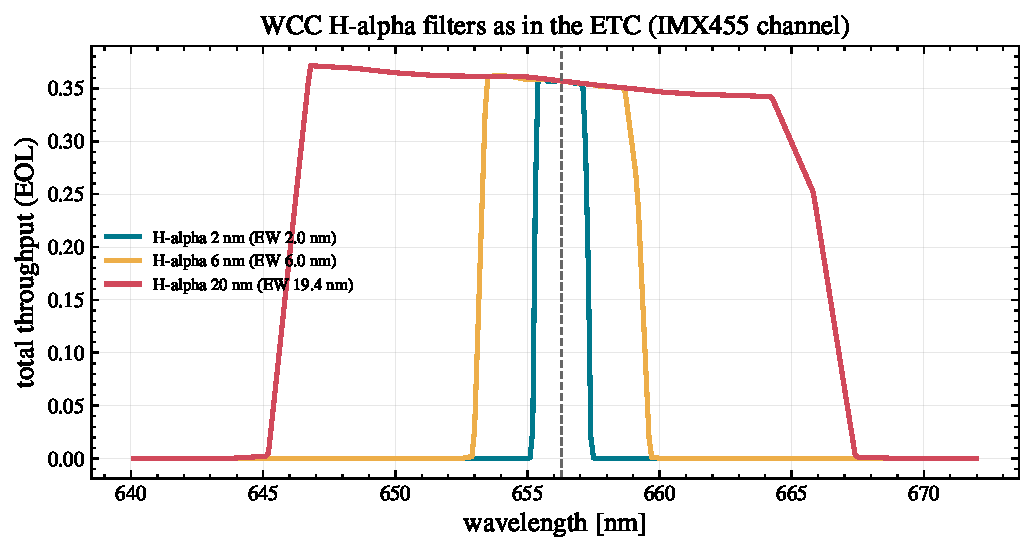
\includegraphics[width=0.6\linewidth]{figures/fig01_filters.pdf}
\caption{End-of-life total throughput of the three WCC \Ha\ filters in the ETC (IMX455 channel), with their equivalent widths. The dashed line is \Ha.}
\label{fig:filters}
\end{figure}

\begin{table}[h!]
\centering\footnotesize
\caption{The three \Ha\ filters for the PDS~70 host (K7V, $G = 11.6$). Rates are detected electrons per second; the planet rate is per $10^{-16}$~\ergcgs\ of line flux. The frame time fills the peak pixel to half the well at 10~mas jitter and $S = 1$. The photon-limited 5$\sigma$ line-flux limit is at 160~mas in 1~h with an ideal PSF subtraction.}
\label{tab:filters}
\begin{tabular}{@{}l r r r r r r@{}}
\toprule
Filter & EW [nm] & Star [e$^-$ s$^{-1}$] & Planet [e$^-$ s$^{-1}$] & Contrast per $10^{-16}$ & Frame [s] & 5$\sigma$ limit [\ergcgs] \\
\midrule
\Ha\ 2~nm  & 2.00  & $1.23 \times 10^4$ & 0.87 & $7.1 \times 10^{-5}$ & 7.6  & $0.83 \times 10^{-16}$ \\
\Ha\ 6~nm  & 5.97  & $3.78 \times 10^4$ & 0.87 & $2.3 \times 10^{-5}$ & 2.5  & $1.45 \times 10^{-16}$ \\
\Ha\ 20~nm & 19.38 & $1.23 \times 10^5$ & 0.87 & $7.1 \times 10^{-6}$ & 0.75 & $2.6 \times 10^{-16}$ \\
\bottomrule
\end{tabular}
\end{table}

\begin{figure}[h!]
\centering
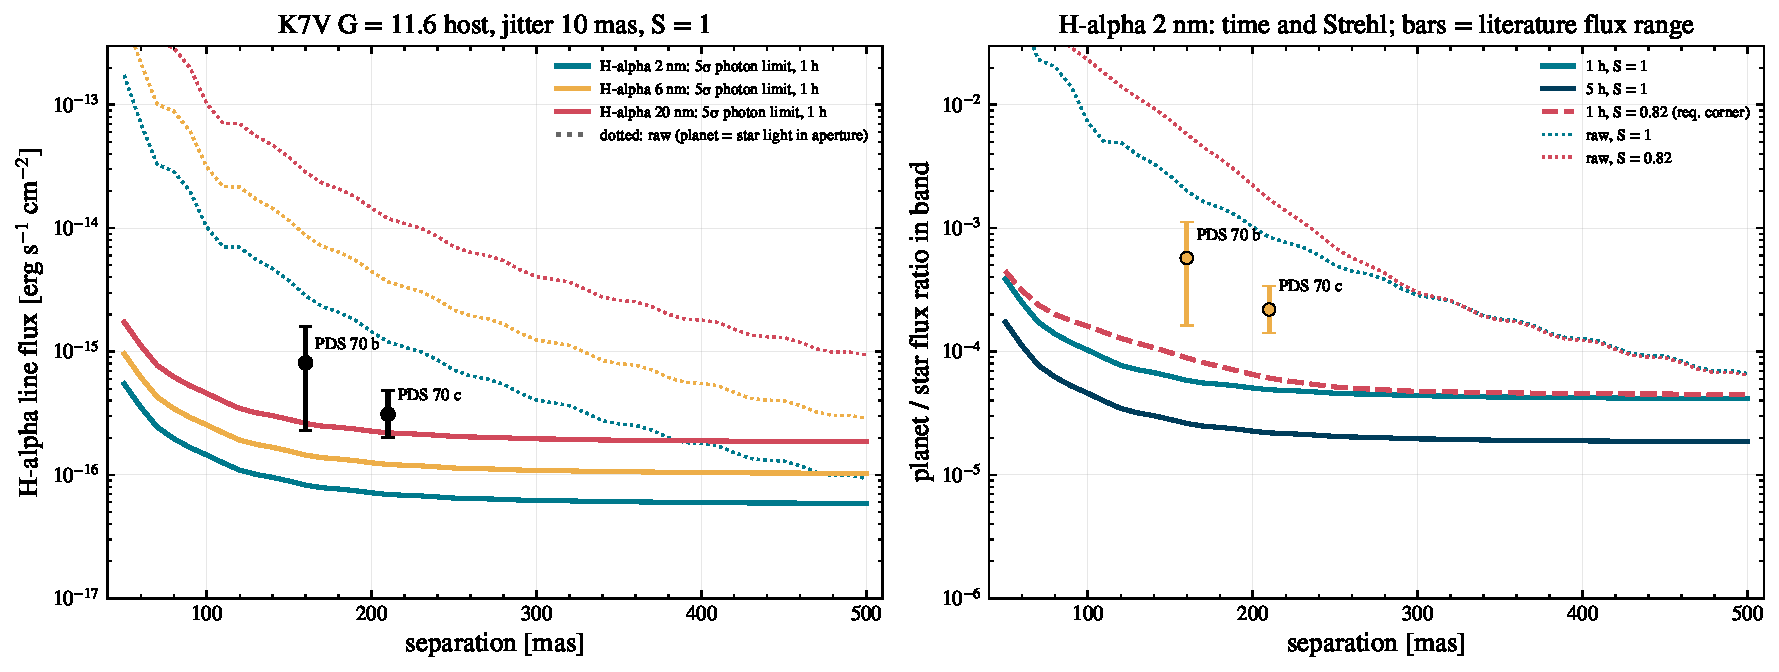
\includegraphics[width=\linewidth]{figures/fig03_contrast_curves.pdf}
\caption{Left: 5$\sigma$ line-flux limit in 1~h (solid) and raw no-subtraction threshold (dotted) versus separation for the three filters, baseline PSF, with PDS~70~b and c and their literature flux ranges. Right: the 2~nm filter as a planet-to-star ratio for 1 and 5~h at $S = 1$ and for 1~h at the requirement corner $S = 0.82$ (dashed), with the raw thresholds dotted.}
\label{fig:contrast}
\end{figure}

\paragraph{Host PSF and contrast curves.} At 656~nm the Airy FWHM is 45.4~mas (2.7~pixels). The jitter-smeared Airy wing at 160~mas holds $1.1 \times 10^{-4}$ of the stellar flux per pixel (1.4~e$^-$~s$^{-1}$ per pixel for the PDS~70 host in the 2~nm filter) and $0.6 \times 10^{-4}$ at 210~mas; the FRED halo is $2 \times 10^{-10}$ per pixel there. In the optimal 2~pixel aperture at 160~mas the stellar light carries 51\% of the variance and read noise 49\% (476 frames of 7.6~s in 1~h); sky and dark are negligible. The 5$\sigma$ limit at 160~mas is $5.8 \times 10^{-5}$ of the stellar flux in the 2~nm band, or $0.83 \times 10^{-16}$~\ergcgs\ (Figure~\ref{fig:contrast}). Because the read-noise term scales with the star as the frame time does, the limit depends on the detector gain mode: a read noise of 1.5~e$^-$ instead of 3.0 improves it by 21\%, 5~e$^-$ degrades it by 35\%, and filling the well to 80\% instead of 50\% improves it by 10\%. The raw threshold (planet equal to the stellar light in the aperture) is $2.0 \times 10^{-3}$ at 160~mas, a factor 3.5 above the ratio of PDS~70~b.

\paragraph{PDS~70.} Table~\ref{tab:pds70} gives the adopted fluxes and the resulting SNR. In the 2~nm filter planet b reaches SNR 19 in 10~minutes and 46 in 1~h at the baseline PSF (31 at the requirement corner); planet c reaches 9 and 22 (18). The 20~nm filter needs 1~h for SNR 15 and 7. At the low end of the observed flux range ($2.3 \times 10^{-16}$ for b, its 2023 state) the 2~nm filter still gives SNR 13 in 1~h.

\begin{table}[h!]
\centering\small
\caption{PDS~70 planets: adopted separations and \Ha\ line fluxes (\ergcgs), one source per number, and the photon-limited SNR in the 2~nm filter with an ideal PSF subtraction, at the baseline PSF (10~mas, $S = 1$) and at the requirement corner ($S = 0.82$). MUSE and MagAO-X measure a pure line flux; HST F656N is line plus continuum in a 1.8~nm band, so part of the range is method rather than variability.}
\label{tab:pds70}
\footnotesize
\begin{tabular}{@{}l l l l l r r@{}}
\toprule
 & Sep.\ used [mas] & Nominal flux & Low & High & SNR 1~h & SNR, $S = 0.82$ \\
\midrule
b & 160 (150--158, C25) & $8.1 \times 10^{-16}$ (H20) & $2.3 \times 10^{-16}$ (C25) & $1.6 \times 10^{-15}$ (Z21) & 46 & 31 \\
c & 210 (207, C25) & $3.1 \times 10^{-16}$ (H20) & $2.0 \times 10^{-16}$ (C25) & $4.8 \times 10^{-16}$ (C25) & 22 & 18 \\
\bottomrule
\end{tabular}
\par\vspace{2pt}\footnotesize Separations in parentheses are the 2023--24 measurements. H20: Hashimoto et al.\ (2020), MUSE 2018. Z21: Zhou et al.\ (2021), HST 2020. C25: Close et al.\ (2025), MagAO-X 2022--2024.
\end{table}

\paragraph{Generic hosts.} For a K7 host of $G = 9$, 11 and 13 the 2~nm 5$\sigma$ limit in 1~h at 200~mas is 2.4, 0.94 and $0.38 \times 10^{-16}$~\ergcgs, and at 100~mas 4.8, 1.9 and $0.76 \times 10^{-16}$ (Figure~\ref{fig:grid}). Brighter hosts are worse twice over: more stellar light in the aperture and shorter frames, hence more read noise; a $G = 9$ host needs 0.7~s frames in the 2~nm filter and 0.07~s in the 20~nm filter, the latter beyond a full-frame readout.

\begin{figure}[h!]
\centering
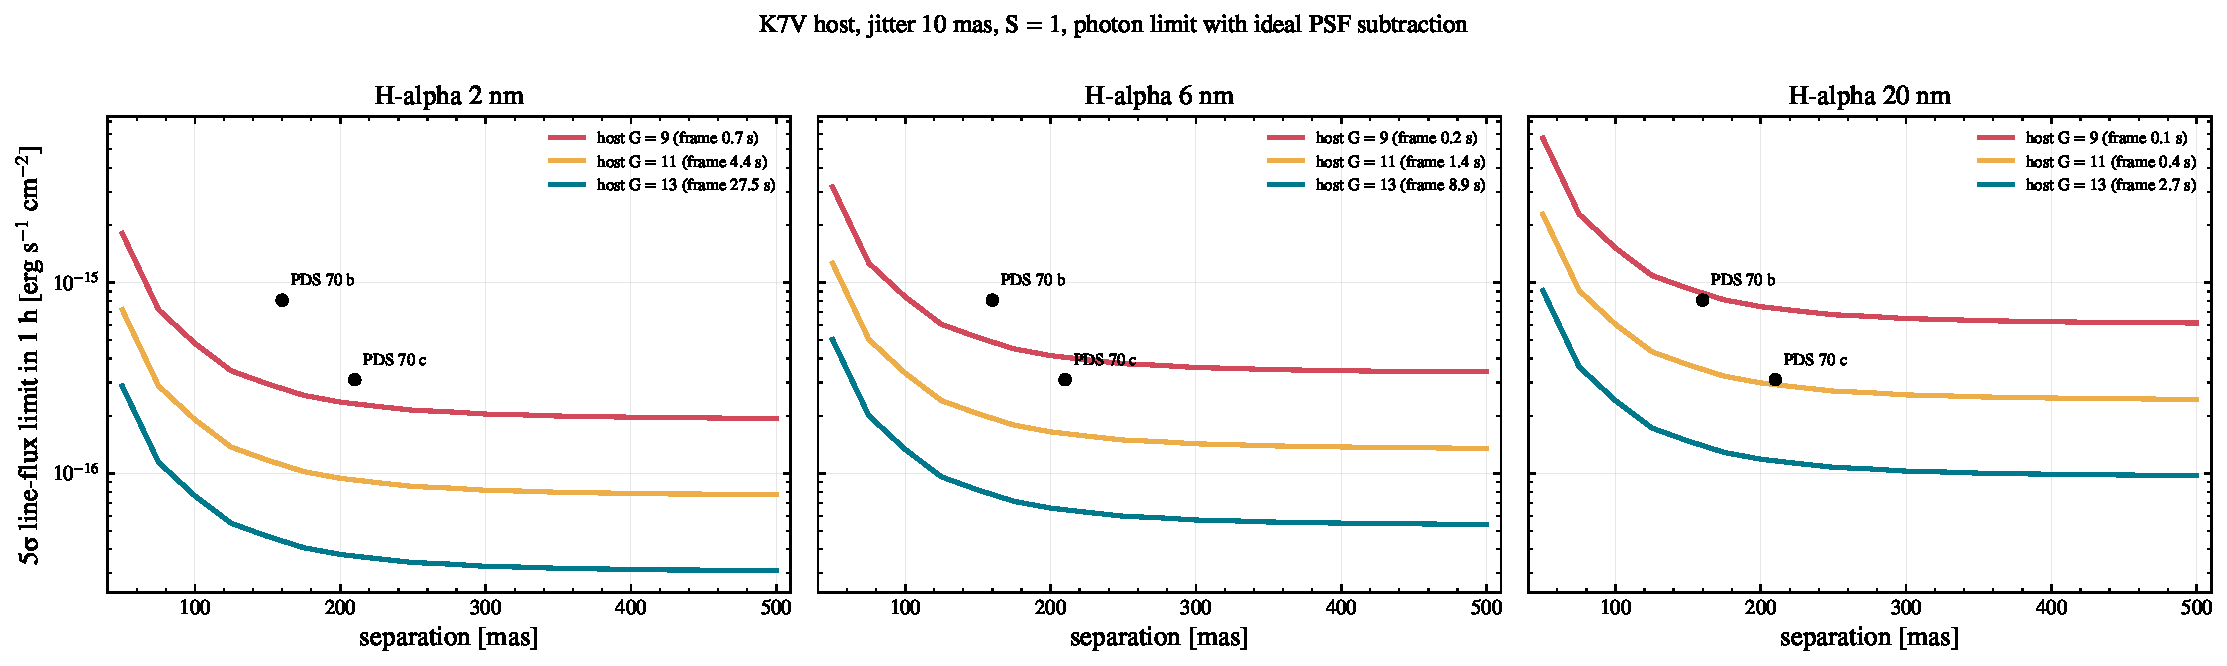
\includegraphics[width=\linewidth]{figures/fig05_fluxlimit_grid.pdf}
\caption{5$\sigma$ \Ha\ line-flux limit in 1~h versus separation for K7 hosts of $G = 9$, 11 and 13 in the three filters, baseline PSF, photon limit with ideal subtraction. Black points are PDS~70~b and c.}
\label{fig:grid}
\end{figure}

\paragraph{Static jitter and Strehl.} Table~\ref{tab:static} gives the stellar light in the 2~pixel aperture at 160~mas for the two Strehl models, relative to the diffraction-limited baseline. The Gaussian halo with $k = 4$ puts 2.4 times the baseline light at $S = 0.82$; a power-law wavefront of the same Strehl puts 1.6 times, and the Gaussian with $k = 2$ 0.86 times (its halo sits inside 100~mas and the renormalization removes light from the wing). The static grid uses the Gaussian model and is therefore on the conservative side. The 5$\sigma$ photon limit at 160~mas relative to the baseline is 0.91 at zero jitter, 1.24 at 20~mas, 1.53 at the requirement corner, 1.95 at 20~mas with $S = 0.82$ and 2.5 at 20~mas with $S = 0.7$ (Figure~\ref{fig:static}); at 300~mas the whole grid stays within 1.25. Jitter of 20~mas raises the aperture light at 160~mas by 11\% and lowers the peak-pixel fraction from 0.087 to 0.053, so the frame time grows from 7.6 to 12.4~s.

\begin{table}[h!]
\centering\footnotesize
\caption{Stellar light in a 2~pixel aperture at 160~mas, 10~mas jitter, relative to $S = 1$, for the Gaussian-halo model with halo FWHM $k$ Airy FWHM and for a random power-law ($f^{-2.5}$) wavefront of the same Strehl; and the peak-pixel fraction and frame time of the Gaussian model.}
\label{tab:static}
\begin{tabular}{@{}l r r r r r r@{}}
\toprule
$S$ (656~nm) & WFE [nm] & Gaussian $k=2$ & Gaussian $k=4$ & Gaussian $k=8$ & Power-law WFE & Frame [s] \\
\midrule
1.0   & 0  & 1.00 & 1.00 & 1.00 & 1.00 & 7.6 \\
0.9   & 34 & 0.92 & 1.81 & 1.96 & 1.56 & 8.3 \\
0.822 & 46 & 0.86 & 2.44 & 2.71 & 1.62 & 9.0 \\
0.7   & 62 & 0.77 & 3.43 & 3.88 & 2.55 & 10.4 \\
\bottomrule
\end{tabular}
\end{table}

\begin{figure}[h!]
\centering
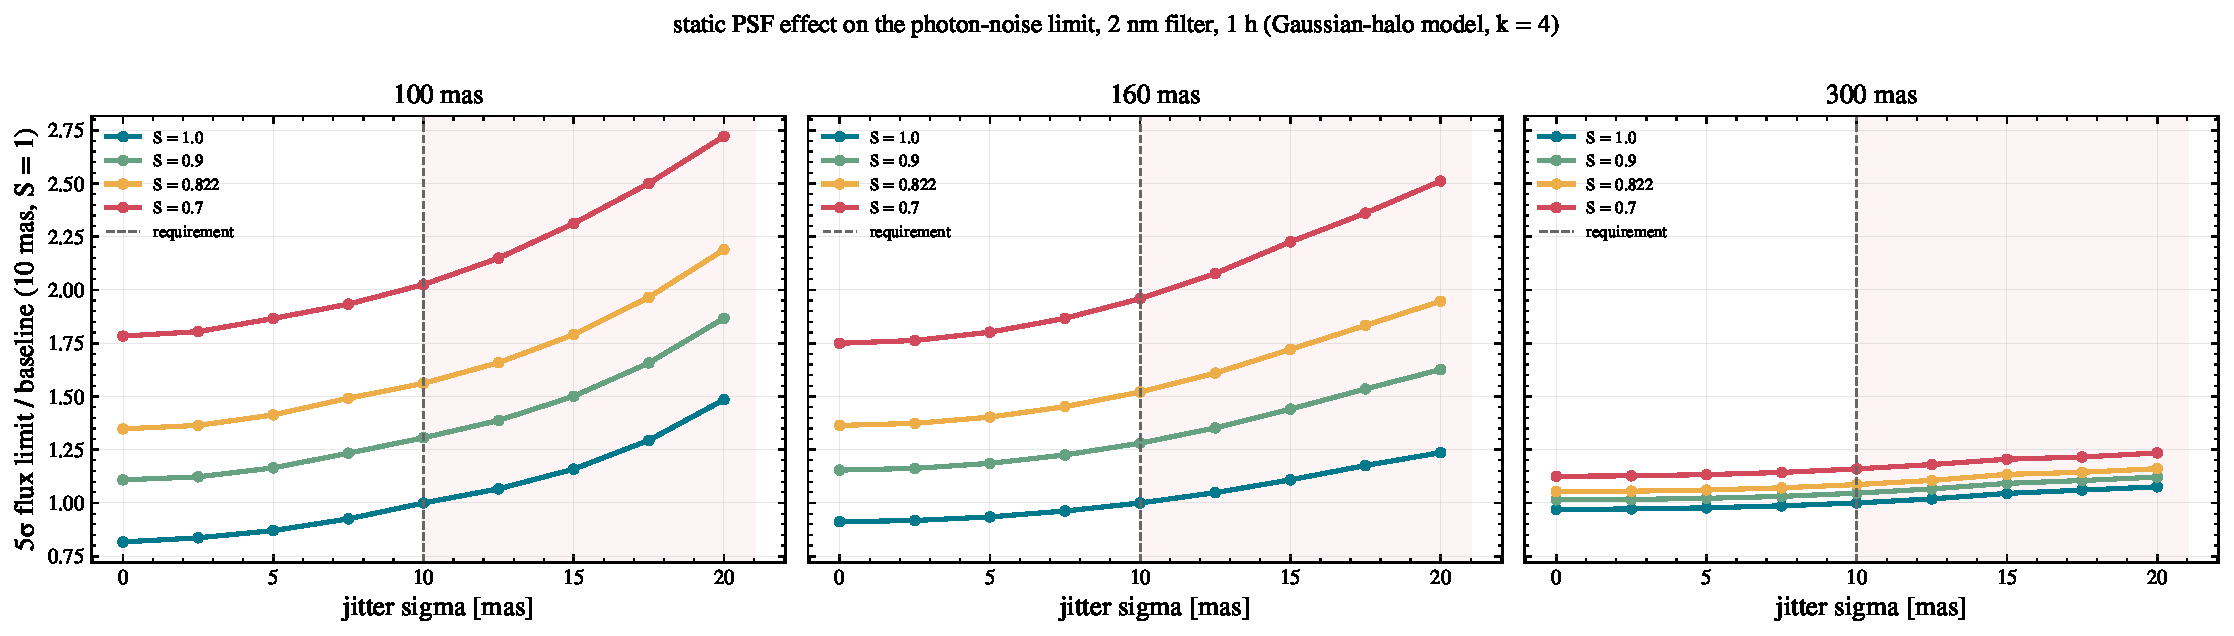
\includegraphics[width=\linewidth]{figures/fig07_js_static_ratio.pdf}
\caption{Photon-limited 5$\sigma$ line-flux limit relative to the baseline (10~mas, $S = 1$) versus jitter for four Strehl values, at 100, 160 and 300~mas, 2~nm filter, 1~h, Gaussian-halo model. The dashed line is the 10~mas requirement and the shaded region is out of specification.}
\label{fig:static}
\end{figure}

\paragraph{Symmetric residuals.} Figure~\ref{fig:symmetric} shows the floor from a 20\% jitter difference between science and reference and from a Gaussian-halo change of $\Delta S = 0.02$, before and after subtracting the azimuthal mean of the residual. Before the fit the jitter term is $1.5 \times 10^{-4}$ at 10~mas and $1.0 \times 10^{-3}$ at 20~mas and the halo term $2 \times 10^{-3}$, all comparable to or above PDS~70~b's ratio of $5.7 \times 10^{-4}$; after the fit both are $1$ to $2 \times 10^{-6}$ up to 15~mas and $9 \times 10^{-6}$ at 20~mas. A residual that is symmetric about the star is not a detection floor for any pipeline that fits a radial profile or scales the reference in an annulus.

\begin{figure}[h!]
\centering
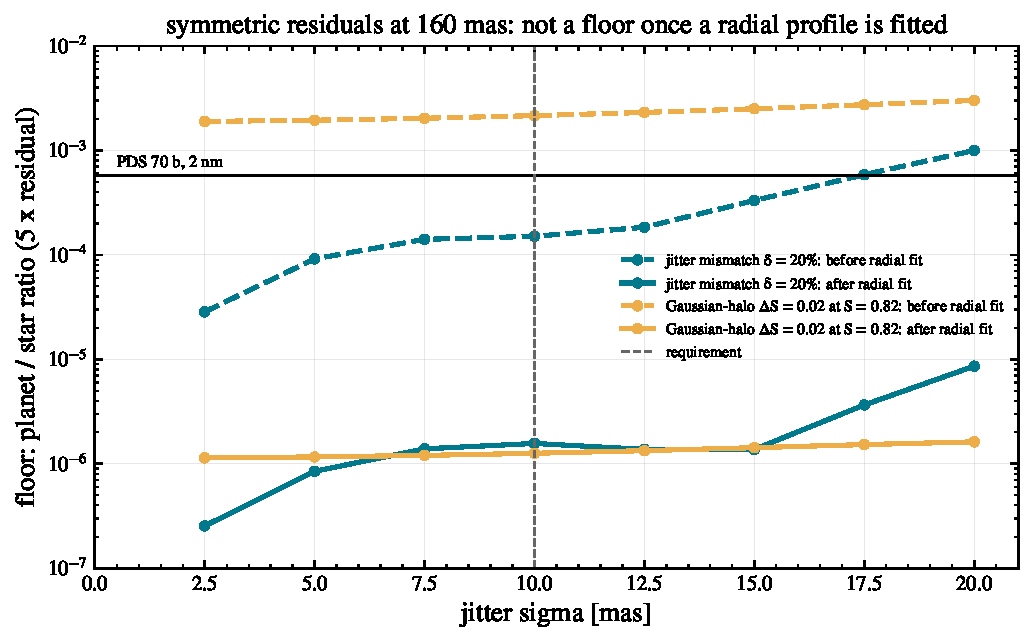
\includegraphics[width=0.62\linewidth]{figures/fig09_js_symmetric_residuals.pdf}
\caption{Symmetric subtraction residuals at 160~mas as a floor (planet flux equal to five times the residual), before (dashed) and after (solid) subtracting the azimuthal mean, for a 20\% jitter mismatch (teal) and a Gaussian-halo Strehl change of 0.02 at $S = 0.82$ (amber). The horizontal line is PDS~70~b in the 2~nm filter.}
\label{fig:symmetric}
\end{figure}

\paragraph{Wavefront drift and registration.} Figure~\ref{fig:asym} shows the asymmetric floors after the radial-profile subtraction. The wavefront-drift floor is linear in the drift amplitude over 0.5 to 8~nm for all three spectra. At 160~mas and a 2.8~nm drift the floor is $4.5 \times 10^{-4}$ (power-law spectrum), $6.7 \times 10^{-4}$ (3 to 5 cycles per aperture) and $1 \times 10^{-5}$ (focus plus astigmatism) at $S = 1$, and $8.9 \times 10^{-4}$, $1.2 \times 10^{-3}$ and $4.0 \times 10^{-4}$ at $S = 0.82$. Expressed as the drift at which the floor equals PDS~70~b in the 2~nm filter: 3.9, 2.4 and 150~nm at $S = 1$; 1.8, 1.3 and 4.0~nm at $S = 0.82$. The low-order term is negligible for perfect optics because focus and astigmatism put light inside 2 Airy FWHM; with 46~nm of static aberration it beats against the static speckles and becomes a first-order term at the planets' separations. The mid-frequency term is nearly independent of the static Strehl because its speckles land on the Airy rings themselves. The registration floor is $8.8 \times 10^{-5}$ for a 0.5~mas shift and $1.8 \times 10^{-4}$ per mas; it equals PDS~70~b at 3.3~mas. Along the separation axis the drift floors fall by a factor 10 between 160 and 300~mas while the photon limit is flat, so beyond 300~mas the problem becomes photon-limited again at the 2.8~nm level.

\begin{figure}[h!]
\centering
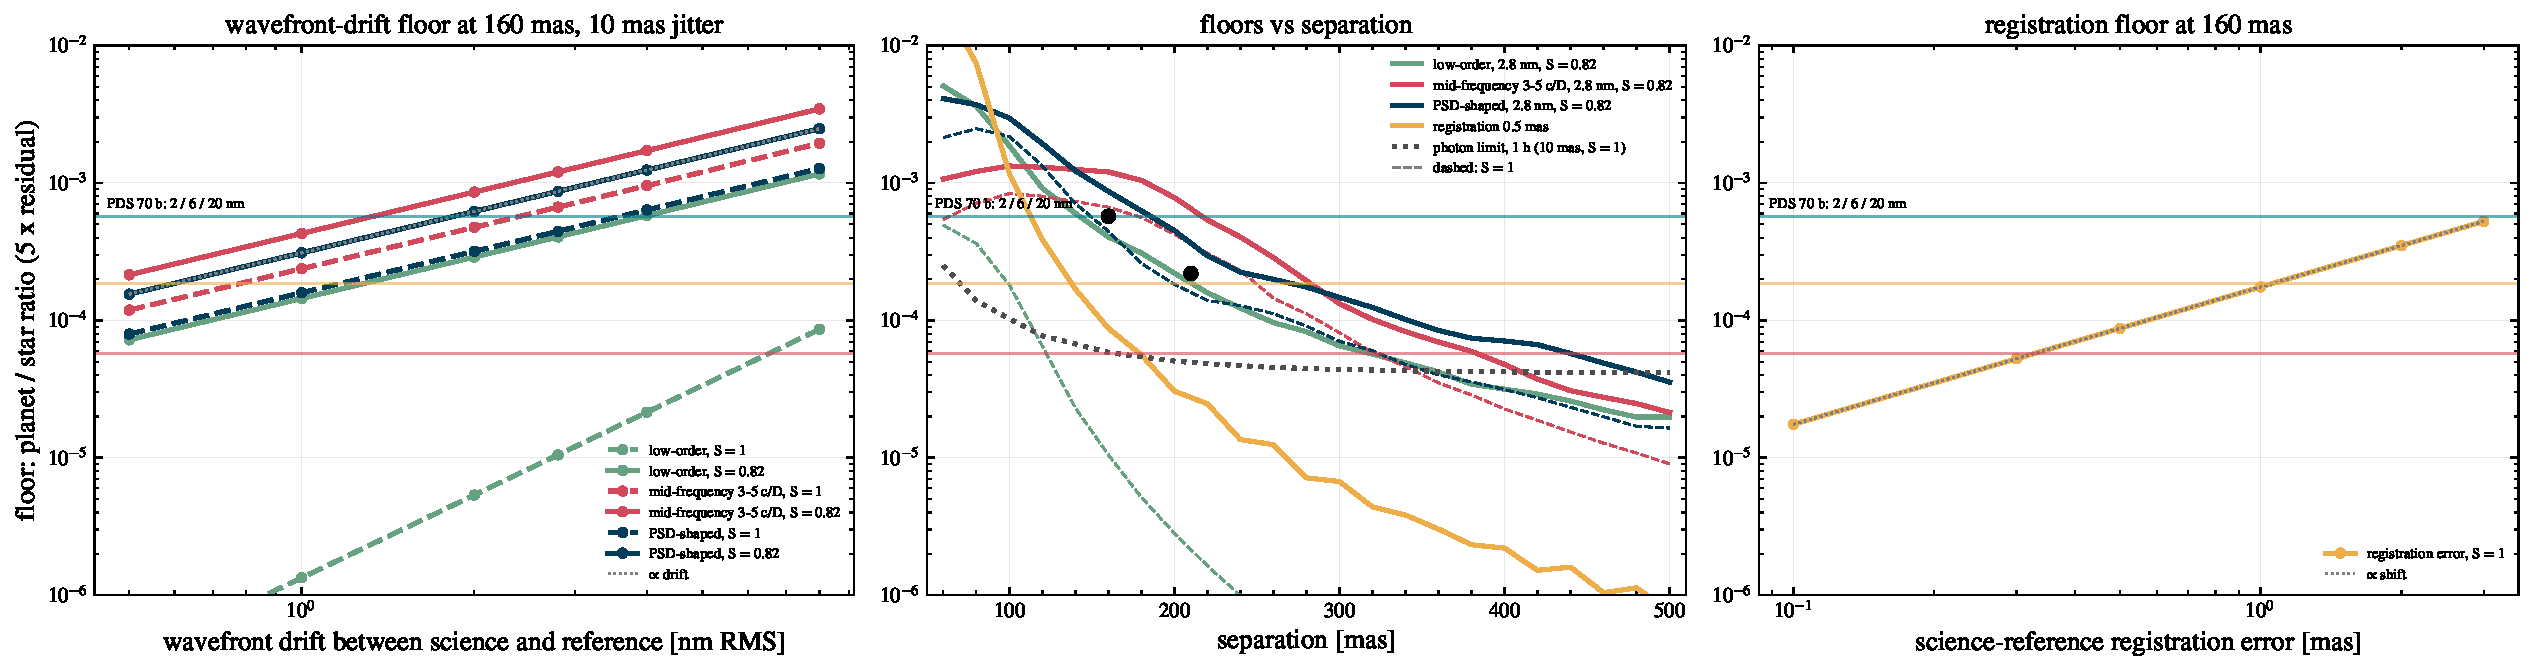
\includegraphics[width=\linewidth]{figures/fig10_js_asymmetric_floors.pdf}
\caption{Asymmetric subtraction floors after a radial-profile fit, as planet-to-star ratio with a 5$\times$ bias margin. Left: floor at 160~mas versus wavefront drift between science and reference for low-order (green), mid-frequency 3 to 5 cycles per aperture (red) and power-law (dark blue) drift spectra, at $S = 1$ (dashed) and $S = 0.82$ (solid). Middle: the same at 2.8~nm versus separation, with the 0.5~mas registration floor (amber) and the 1~h photon limit (dotted). Right: registration floor at 160~mas versus shift. Horizontal lines mark PDS~70~b in the 2, 6 and 20~nm filters.}
\label{fig:asym}
\end{figure}

\paragraph{Combined.} Table~\ref{tab:corners} collects the terms at 160~mas for the corners of the grid, and Figure~\ref{fig:combined} the full grid. With a 2.8~nm power-law drift and a 0.5~mas registration error the detectable flux is 0.7 of PDS~70~b at $S = 1$ for any jitter up to 12.5~mas and 1.5 of it at the requirement corner; the drift term dominates everywhere except at $S = 1$ with 15 to 20~mas jitter, where registration and drift are comparable. The allowed drift at the requirement corner is 1.9~nm RMS (power-law spectrum), and it falls to 1.2~nm at $S = 0.7$ with 20~mas jitter.

\begin{table}[h!]
\centering\small
\caption{Detectable \Ha\ line flux at 160~mas for the PDS~70 host in the 2~nm filter, 1~h, at grid corners (\ergcgs): photon limit with ideal subtraction; floor from a 2.8~nm RMS power-law wavefront drift between science and reference; floor from a 0.5~mas registration error; the largest of the three relative to PDS~70~b's nominal $8.1 \times 10^{-16}$; and the power-law drift at which the floor equals that flux. Floors carry a 5$\times$ bias margin.}
\label{tab:corners}
\begin{tabular}{@{}r r r r r r r@{}}
\toprule
Jitter [mas] & $S$ & Photon & Drift 2.8~nm & Registration 0.5~mas & Limit / $F_{\rm b}$ & Allowed drift [nm] \\
\midrule
0  & 1.00 & $0.75 \times 10^{-16}$ & $5.7 \times 10^{-16}$ & $1.3 \times 10^{-16}$ & 0.70 & 4.0 \\
10 & 1.00 & $0.83 \times 10^{-16}$ & $5.8 \times 10^{-16}$ & $1.2 \times 10^{-16}$ & 0.72 & 3.9 \\
10 & 0.82 & $1.26 \times 10^{-16}$ & $1.18 \times 10^{-15}$ & $1.2 \times 10^{-16}$ & 1.46 & 1.9 \\
20 & 1.00 & $1.02 \times 10^{-16}$ & $7.1 \times 10^{-16}$ & $1.9 \times 10^{-16}$ & 0.88 & 3.2 \\
20 & 0.82 & $1.61 \times 10^{-16}$ & $1.35 \times 10^{-15}$ & $1.9 \times 10^{-16}$ & 1.66 & 1.7 \\
20 & 0.70 & $2.07 \times 10^{-16}$ & $1.83 \times 10^{-15}$ & $1.9 \times 10^{-16}$ & 2.26 & 1.2 \\
\bottomrule
\end{tabular}
\end{table}

\begin{figure}[h!]
\centering
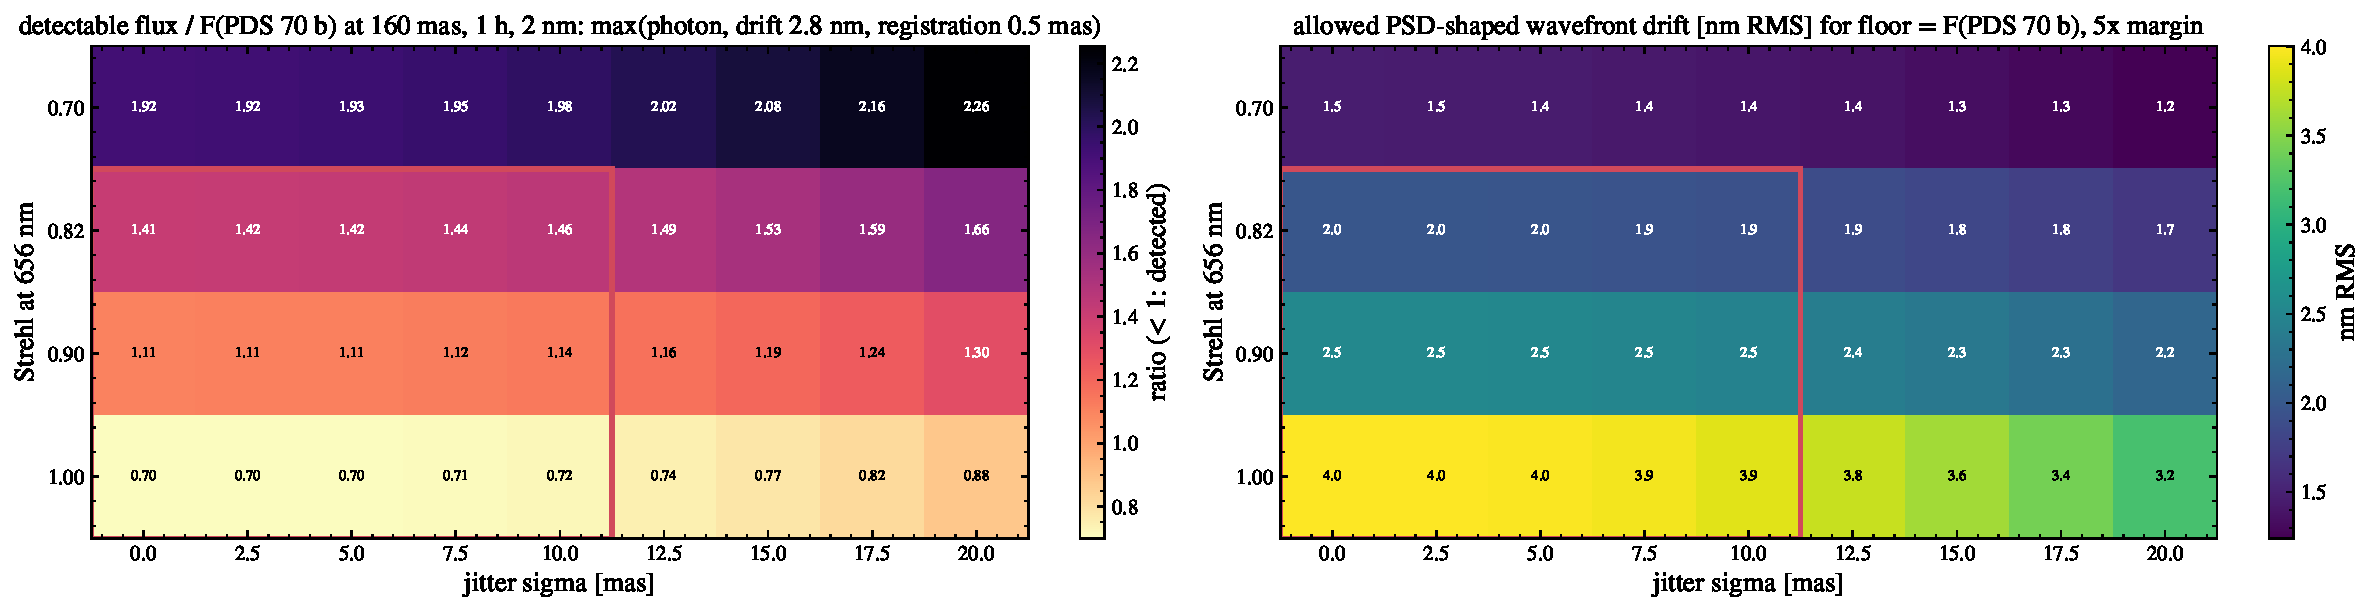
\includegraphics[width=\linewidth]{figures/fig12_js_combined.pdf}
\caption{Left: detectable line flux at 160~mas in 1~h relative to PDS~70~b, taking the largest of the photon limit, the 2.8~nm power-law drift floor and the 0.5~mas registration floor, over the jitter and Strehl grid; the red box is jitter $\le 10$~mas and $S \ge 0.82$. Right: the power-law wavefront drift between science and reference at which the floor equals PDS~70~b's flux.}
\label{fig:combined}
\end{figure}

% ============================================================================
\section*{Discussion}

\paragraph{What the numbers say.} The WCC has the collecting area and the pixel scale to detect the PDS~70 planets in \Ha\ in an hour of stacked frames, provided the stellar PSF can be subtracted to a small fraction of its own wing. The photon budget is not the issue. Neither, for this science, are the jitter and Strehl values under discussion: across the whole grid the static effect on the photon limit at the planets' separations is a factor 0.9 to 2.5. What sets the floor is how well two PSFs taken at different times match after a radial-profile fit, and that is controlled by the wavefront repeatability in nanometers, the registration in fractions of a milliarcsecond, and the spatial frequencies involved. The requirement conversation for this case should therefore be about PSF stability, not PSF quality.

\paragraph{Why the filter matters twice.} The photon-limited gain of the 2~nm filter is only the square root of the bandwidth ratio, because every term in the noise, including read noise through the frame time, scales with the stellar rate. The systematic floors do not average down and are a fixed fraction of the stellar light, so against them the narrow filter buys the full factor 10 over the 20~nm filter and 3 over the 6~nm filter. A real observation will be systematics-limited at the 160 to 200~mas separations of the PDS~70 planets, so the 2~nm filter is the one that makes the science possible rather than merely faster. Its 7.6~s frames also keep the readout duty cycle near unity, where the 20~nm filter's 0.75~s frames would lose about a third of the time.

\paragraph{Wavefront drift as a requirement.} A drift of 2 to 4~nm RMS between science and reference is the level at which PDS~70~b becomes marginal with a 5$\times$ margin; the raw residual equals the planet at 10 to 20~nm. Which of these applies depends on the pipeline. The 5$\times$ margin is the conservative reading for a single reference; a roll pair, a library of references or a forward-modelled subtraction would recover part of it. The spatial-frequency dependence is the useful content for engineering: focus and astigmatism drift (thermal breathing) is harmless for a diffraction-limited telescope and costs only through the static aberrations it beats against, so a static wavefront error budget of 46~nm makes a 4~nm low-order drift matter where 150~nm would not. Drift at 3 to 5 cycles per aperture (segment or support-print-through scales for a 3~m primary) is the most damaging per nanometer and is the term to hold tightest. These numbers should be read as the drift over the interval between the science and reference sequences, not over a mission; a reference taken within the same thermal state, or a spacecraft roll between two halves of the same visit, is the operational way to meet them.

\paragraph{Model dependence.} The static Strehl penalty depends on where the aberrated light lands. The Gaussian halo with $k = 4$, inherited from the companion memo, is conservative by a factor 1.5 in stellar light at the requirement Strehl relative to a power-law wavefront; had the grid been run with the power-law PSF the static factors in Table~\ref{tab:static} would be closer to 1.3 than 1.5 at the requirement corner. The drift floors are computed with the power-law PSF and random screens (mean of three realizations), and their linear scaling with drift is exact to first order, so the allowed-drift values are robust to the amplitude chosen; they are less robust to the assumed spectral shape, which is why three shapes are given.

\paragraph{Limitations.} The stellar PSF is the ETC's unobscured circular-aperture Airy pattern; a central obstruction would raise the ring envelope at 3 to 5 Airy FWHM by up to a factor of two in stellar light and shift the ring phases, which would move the photon limit by up to 1.4 and leave the systematic ratios unchanged. The PSF is monochromatic; across the 2~nm band the radial smear at 160~mas is 0.5~mas, negligible, and across 20~nm it is 5.5~mas, which softens the rings for that filter only. Near-core scattered light from micro-roughness or particulates is not in the FRED map inside 1.4$^{\prime\prime}$ and is not modeled here. The host's own \Ha\ emission is small for PDS~70 (the HST cross-check bounds it at the 10\% level) but would double the stellar light in the 2~nm band for a classical T~Tauri host with an equivalent width of tens of \AA. Saturation is a half-well rule with no nonlinearity, bleeding or persistence; a reference-scaling error from detector nonlinearity or host variability adds a symmetric term of $7 \times 10^{-5}$ per percent at 160~mas before an annulus fit removes it. The floors are single-parameter and coherent; a real subtraction combines them and partly averages them. The planet fluxes are variable by factors of a few and PDS~70~b was in a faint state in 2023 to 2024.

\paragraph{Recommendations.} (1) Adopt the 2~nm \Ha\ filter as the baseline for protoplanet imaging and keep its end-of-life peak throughput at the level of the wider filters. (2) Add a WCC PSF-stability requirement for this mode, expressed as the wavefront repeatability between a science and a reference sequence in nm RMS per spatial-frequency band, with Table~\ref{tab:corners} and Figure~\ref{fig:combined} as the trade space; the 10~mas jitter and $S = 0.8$ requirements do not need tightening for this case. (3) Ask the stray-light analysis for a near-core (0.1 to 1$^{\prime\prime}$) scatter estimate, which no current model provides. (4) Plan the observing mode around PSF repeatability: reference star or roll pair within the same thermal state, sub-milliarcsecond frame registration, and a radial-profile or annulus-scaled subtraction as the minimum pipeline. (5) Before the Science Preliminary Design Review, repeat the drift calculation with the real pupil geometry and a wavefront drift budget from the thermal model, and add a forward-modelled subtraction to quantify how much of the 5$\times$ margin a planet-aware pipeline recovers.

% ============================================================================
\section*{Appendix}

\paragraph{Derivations and conventions.}
\begin{itemize}[leftmargin=*]
  \item Airy FWHM: $1.028\,\lambda/D = 45.4$~mas at 656.3~nm for $D = 3.065$~m; 2.69 pixels at 16.87~mas per pixel.
  \item Mar\'echal: $S = \exp[-(2\pi\sigma_{\rm wfe}/\lambda)^2]$. $S = 0.8$ at 615~nm is 46~nm RMS and gives $S = 0.82$ at 656~nm; $S = 0.9$, 0.8 and 0.7 at 656~nm are 34, 49 and 62~nm RMS.
  \item Line rate: the ETC integrates the Gaussian line through the filter and detector throughput; $10^{-16}$~\ergcgs\ gives 0.87~e$^-$~s$^{-1}$ in every \Ha\ filter. The K7V host at $G = 11.6$ gives the rates in Table~\ref{tab:filters}.
  \item Frame time: $t_{\rm frame} = 0.5\,W / (F_\star\,p)$ with $W$ the well depth, $F_\star$ the stellar rate and $p$ the peak-pixel fraction of the rendered PSF.
  \item Photon limit: $F_{\rm lim} = 5\,\sqrt{F_\star f_\star T + (B + D)\,N_{\rm pix} T + N_{\rm frame}\,\sigma_{\rm rn}^2 N_{\rm pix}}\,/\,(f_{\rm p} T)$, converted to line flux with the line rate above; $f_\star$ is the stellar PSF fraction in the aperture at the planet's separation, $f_{\rm p}$ the planet's enclosed fraction, $N_{\rm pix} = \pi r_{\rm ap}^2$, and the aperture radius is chosen to minimize $F_{\rm lim}$. Because $t_{\rm frame} \propto 1/F_\star$, the read-noise term scales with $F_\star$ like the photon term, and the limit scales as $\sqrt{F_\star}$, i.e., as the square root of the filter width.
  \item Raw contrast: $f_\star / f_{\rm p}$.
  \item Subtraction floor: $5\,\langle (f_{\star,{\rm sci}} - f_{\star,{\rm ref}})^2 \rangle^{1/2} / f_{\rm p}$, with the average over seven separations spanning $\pm$22.7~mas around the quoted one, in a 2~px aperture.
\end{itemize}

\paragraph{Provenance.} Instrument model: \texttt{wcc\_etc} (Lazuli configuration: $D = 3.065$~m, $f/15$, jitter 10~mas, IMX455 read noise 3.0~e$^-$, dark 0.003~e$^-$~s$^{-1}$, well 16.3~ke$^-$ at the ETC gain setting), \Ha\ filter curves \texttt{wcc\_imx\_Ha\_\{2,6,20\}nm\_EOL.csv}. FRED stray-light map: run 26-0212 at 450~nm, via \texttt{wcc\_sim.scatter}. Planet fluxes and separations: stated values from the references below (Table~\ref{tab:pds70}); all contrast numbers are derived here. The requirement values (10~mas jitter, Strehl 0.8 at r) are the working values under discussion and are not taken from a released requirements document. The wavefront-drift and registration levels are scenarios, not measured spacecraft properties; the floors scale linearly with them.

\paragraph{Reproduction.}
\begin{itemize}[leftmargin=*]
  \item \texttt{wcc-sim/notebooks\_scrap/halpha\_hci\_feasibility.ipynb} and \texttt{halpha\_hci\_jitter\_strehl.ipynb}, built from \texttt{build\_halpha\_hci\_*.py} and executed in the \texttt{py313} environment (about 1.5~minutes each). Figures and machine-readable tables (\texttt{*.ecsv}) are in \texttt{notebooks\_scrap/halpha\_hci\_out/}.
  \item Shared helpers with self-checks: \texttt{notebooks\_scrap/hci\_psf.py} (\texttt{python hci\_psf.py}).
\end{itemize}

\paragraph{References.}
\begin{itemize}[leftmargin=*]
  \item Haffert, S.~Y., et al.\ 2019, Nature Astronomy, 3, 749, \url{https://doi.org/10.1038/s41550-019-0780-5}: discovery of \Ha\ emission from PDS~70~b and c with VLT/MUSE; distance 113.43~pc; c at 240~mas in 2018.
  \item Hashimoto, J., et al.\ 2020, AJ, 159, 222, \url{https://doi.org/10.3847/1538-3881/ab811e}: MUSE line fluxes $8.1 \pm 0.3 \times 10^{-16}$ (b) and $3.1 \pm 0.3 \times 10^{-16}$~\ergcgs\ (c). Source of the nominal fluxes in Table~\ref{tab:pds70}.
  \item Zhou, Y., et al.\ 2021, AJ, 161, 244, \url{https://doi.org/10.3847/1538-3881/abeb7a}: HST WFC3 F656N line flux of b, $1.62 \pm 0.22 \times 10^{-15}$~\ergcgs, separation $177.0 \pm 9.4$~mas, stellar F656N flux $1.18 \times 10^{-12}$~\ergcgs, variability below 30\% over five months. Source of the upper end of the b range and of the host cross-check.
  \item Close, L.~M., et al.\ 2025, AJ, 169, 35, \url{https://doi.org/10.3847/1538-3881/ad8648}: MagAO-X \Ha\ imaging 2022--2024; b at $(10.4 \pm 1.6)$, $(2.28 \pm 0.26)$ and $(3.64 \pm 0.87) \times 10^{-16}$~\ergcgs\ at 158, 157 and 150~mas; c at $(3.3 \pm 1.5)$, $(2.04 \pm 0.21)$ and $\sim\!4.8 \times 10^{-16}$~\ergcgs\ at 218, 206 and 207~mas; ground-based 5$\sigma$ contrast of $10^{-4}$ at 200~mas. Source of the lower end of the b range and of the separations used here.
  \item Mar\'echal, A., 1947, Rev.\ Opt., 26, 257; Mahajan, V.~N., 1983, JOSA, 73, 860, \url{https://doi.org/10.1364/JOSA.73.000860}: Strehl versus wavefront-error approximation and its validity range.
\end{itemize}

\end{document}
